%==============================================================================
\chapter{Introduction}
%------------------------------------------------------------------------------

The digital CMS pixel chip, colloquially called \glsreset{ROC}\gls{ROC}, consists of 52$\times$80~\gls{PUC}. Electrically they are organized in 26~\gls{DC}, each having 2$\times$80~pixels. One double column is controlled by a periphery which has buffers for time-stamps and data. There are 24~time-stamp buffers (8~bit wide) and 80~data buffers, see Fig.~\ref{fig:ROCimage}

\begin{figure}[hbtp]
	\begin{center}
	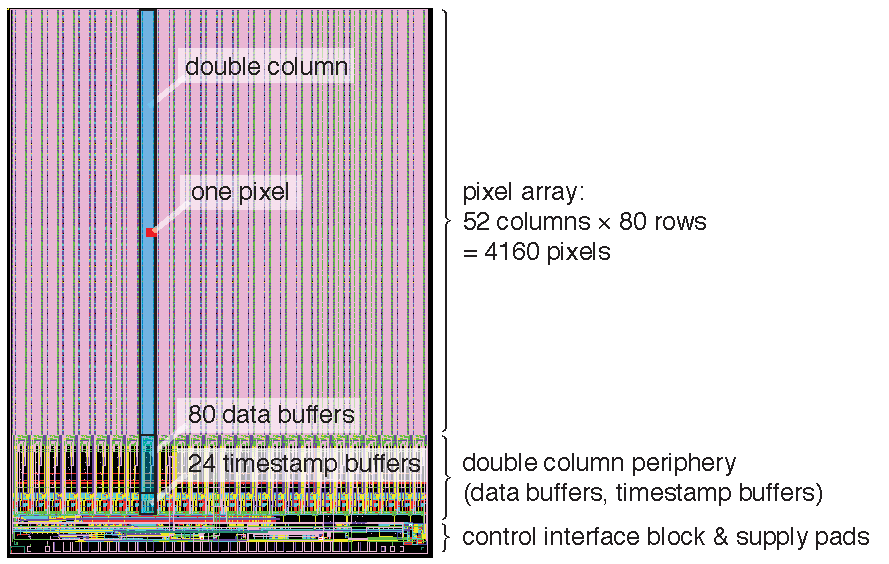
\includegraphics[width=.9\textwidth]{img/ROCimage.pdf}
	\end{center}
	\caption{Pixel chip arrangement. The image shows the full layout of a pixel chip. Highlighted are the areas of a single pixel, double column, the data buffers and the timestamp buffers. The periphery and the supply pads are in charge to handle trigger information, buffer data of recent pixel data and handle the communication with the outer world.}
	\label{fig:ROCimage}
\end{figure}



